\section{Introduction}\label{sec1}

Nowadays, in which the use of both natural and artificial resources is essential,
it is necessary an exhaustive schedule to make the best use of these resources. Scheduling is part of the project management of any organization, regardless of its size and context.
This topic has become so relevant that there is even a publication exclusively dedicated to it called the \emph{Journal of Scheduling}, with a JCR impact factor (Q3) and is indexed by Scopus and has a Cite Score of 3.7 for 2021 ~\cite{JournalSchedul2003}.
%%% Web de Journal of Scheduling  https://www.springer.com/journal/10951
Furthermore, there are recent systematic reviews on schedule such as Fernandes et al. in ~\cite{fernandes2022energy} focused on energy-efficient scheduling in job shop manufacturing
systems. There are numerous types of deterministic scheduling problems, in Blazewicz et al.~\cite{blazewicz2019handbook} they are classified according to several criteria: processors used, task and resource characteristics, and optimality (performance measure).
Scheduling problems can be solved from different approaches, but we focus on the techniques of constraint satisfaction in scheduling from the Artificial Intelligence point of view \cite{bsr10}.\\


Scheduling problems are well suited to be solved by constraint programming (CP) and its associated systems~\cite{CANIZARES2022}. 
Among the software that implements scheduling problems, 
in this paper we have used MiniZinc~\cite{ nethercote2007minizinc}, an open source constraint modeling language. In particular, we studied several examples of scheduling problems implemented in MiniZinc. 
For testing these programs that implement scheduling problems, MT will be used.\\

MT is a software testing technique that is based in MRs \cite{segura2011automated}.
An MR is a relationship defined between multiple inputs and outputs that is met. 
The goal is obtaining (by MRs) new test cases (follow-up test cases named) that detect errors that original test cases did not detect. Chen introduced this name in~\cite{chen1998metamorphic}, it has been applied to numerous contexts and programs. A specific event is held annually~\cite{ 7961643,Xie:2019:3340651} from 2016. 
An example of the usefulness of MRs is given as follows. Consider, for example, a program SP, which implements the computation of the shortest path between any two nodes $a$, and $b$, $SP(G,a,b)$. For testing whether the solution is correct, we can obtain another test case, in which the path is in reverse order $SP(G,b,a)$. Therefore, it must be satisfied that $SP(G,a,b)= SP(G,b,a)$. If the results are different, we have detected a failure in the program. This MR can be defined in general terms as: 
$MR: \forall x, y \in G, SP(G, x,y) = SP(G, y,x) $
Despite the fact that MT has been applied to multiple domains and programs ~\cite{Chen:2018:MTR:3177787.3143561,almendros2021metamorphic}, its application to programs that implement scheduling problems implemented in MiniZinc constraint language is a novel proposal. Hence, Minizinc has been applied to support MT~\cite{de2019using}.\\

% Esta figura está inspirada en https://www.researchgate.net/figure/METtester-Architecture_fig2_326048835
%%% [htb!]
\begin{figure*}[h!]
    \centering
    %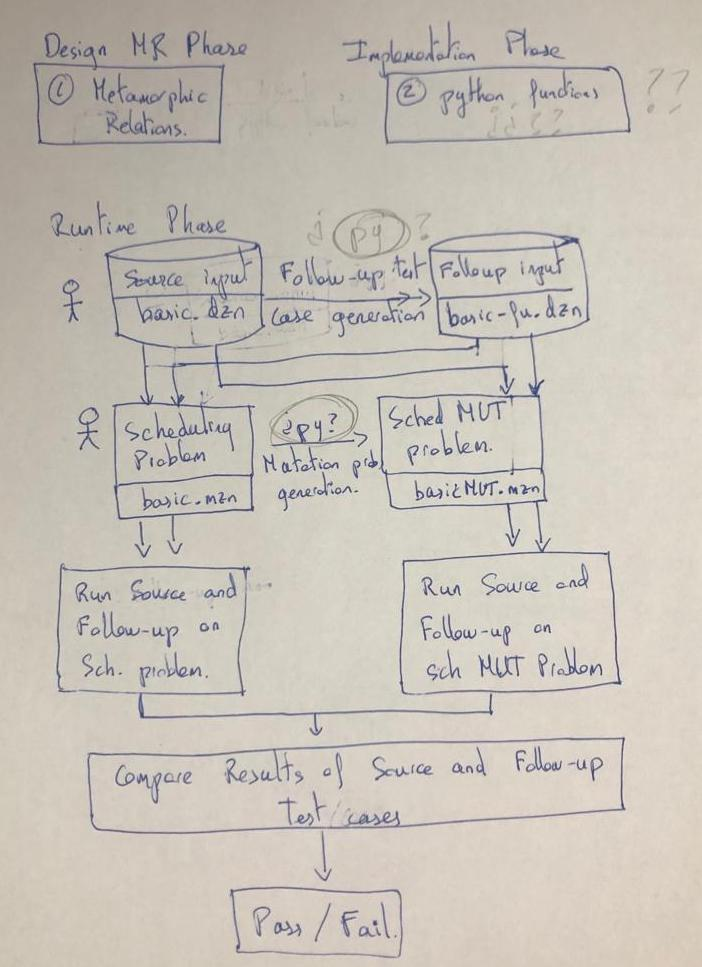
\includegraphics[scale=0.4]{Figures/boceto.jpeg}
    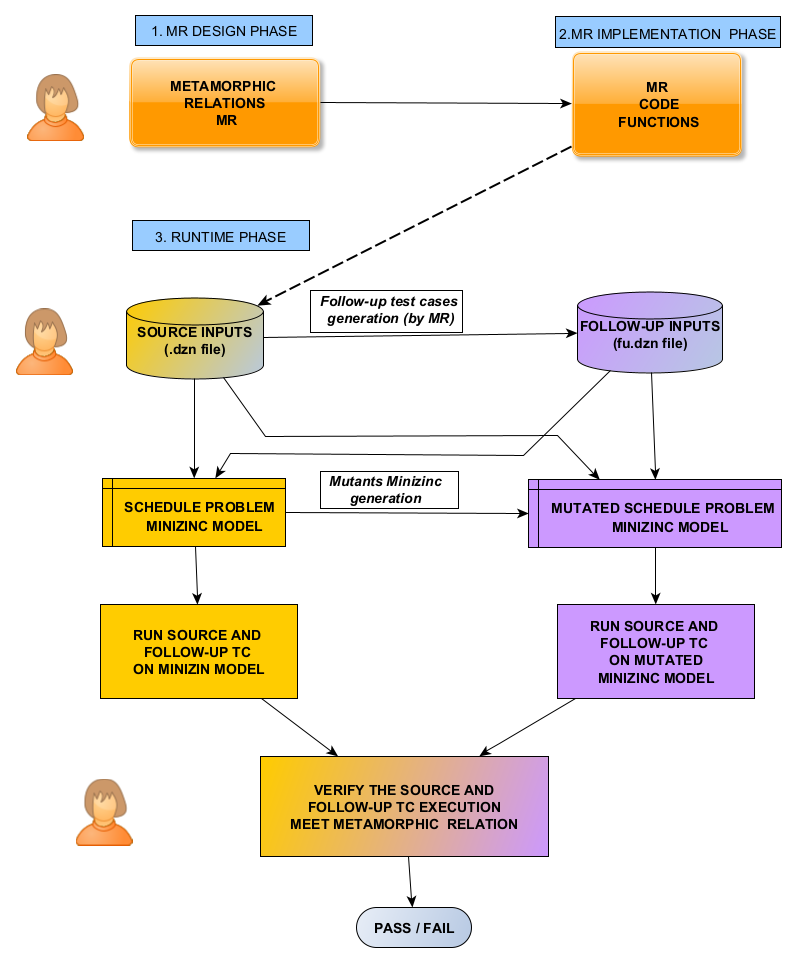
\includegraphics[scale=0.85,width=0.7\textwidth]{Figures/SCHEDUL_MR_MZ_ARCH.png}
    \caption{Architecture of our scheduling constraint programming metamorphic testing framework}
    \label{fig:MTSchedArch}
\end{figure*}


In this paper, we apply MT to constraint language programs in
MiniZinc that implement scheduling problems. Particularly, we consider some 
examples of this type of programs because they are representative of the 
scheduling problems implemented in MiniZinc. These programs are shown and 
explained in detail in Section~\ref{sec:Empirical Evaluation}. Furthermore, 
we visually represent the architecture scheme of our framework 
in Fig.~\ref{fig:MTSchedArch}. Next, we briefly explain 
each step of the process performed.
\begin{itemize}
    \item \textbf{MR design phase}. A set of MRs have been designed in order to 
    obtain new test cases (follow-up) that detect errors in MiniZinc programs that implement scheduling problems.
    In order to design each MR, the input data to each program have been 
    analyzed to adapt it to them.
    \item \textbf{MR Implementation phase}. Properties (MRs) have been defined on the original test cases to obtain the follow-up test cases. These properties have been implemented as functions on the program input data.
    \item \textbf{Runtime phase}. In this stage: the follow-up test cases are 
    generated by executing the MRs; mutations of the original programs are built 
    in according to different defined mutation operators; then the mutated 
    programs are executed with the original test cases and with the follow-up test cases. 
    Finally, the results are validated, checking if the MRs are met. If any MR is not met, it indicates that the error injected in the mutant has been detected.
\end{itemize}



%% Chen:2018:MTR:3177787.3143561
%%% Segura16
In the following sections we outline, Section~\ref{sec2} describes related work.
Following Section~\ref{sec3} concepts and notations are defined. In  Sections~\ref{sec:metamorfic_relations} and \ref{sec:mutants}, particular MRs and mutation operators are designed and implementation details described. In the Section~\ref{sec:Empirical Evaluation} our approach is evaluated, 
through to research questions, and the results are discussed, as well as the threads to validity are included. At the end, in the Section~\ref{sec6} the conclusions and future work are presented.

% The paper is structured as follow






%Notación: Los ficheros de datos de casos Follow-up se van a notar de la siguiente forma con el átomo fu. Por ejemplo, basic.dzn es basic-fu-all-prec.dzn.


